%\documentstyle[10pt,twoside]{article}
%\documentstyle[twoside]{article}
\documentclass[twoside]{article}
\setlength{\oddsidemargin}{0.25 in}
\setlength{\evensidemargin}{-0.25 in}
\setlength{\topmargin}{-0.6 in}
\setlength{\textwidth}{6.5 in}
\setlength{\textheight}{8.5 in}
\setlength{\headsep}{0.75 in}
\setlength{\parindent}{0 in}
\setlength{\parskip}{0.1 in}

\usepackage{graphicx}
\usepackage{url}


%
% The following commands sets up the lecnum (lecture number)
% counter and make various numbering schemes work relative
% to the lecture number.
%
\newcounter{lecnum}
\renewcommand{\thepage}{\thelecnum-\arabic{page}}
\renewcommand{\thesection}{\thelecnum.\arabic{section}}
\renewcommand{\theequation}{\thelecnum.\arabic{equation}}
\renewcommand{\thefigure}{\thelecnum.\arabic{figure}}
\renewcommand{\thetable}{\thelecnum.\arabic{table}}
\newcommand{\dnl}{\mbox{}\par}

%
% The following macro is used to generate the header.
%
\newcommand{\lecture}[4]{
   \pagestyle{myheadings}
   \thispagestyle{plain}
   \newpage
   \setcounter{lecnum}{#1}
   \setcounter{page}{1}
   \noindent
   \begin{center}
   \framebox{
      \vbox{\vspace{2mm}
    \hbox to 6.28in { {\bf CMPSCI~677~~~Operating Systems
                        \hfill Spring 2017} }
       \vspace{4mm}
       \hbox to 6.28in { {\Large \hfill Lecture #1: #2  \hfill} }
       \vspace{2mm}
       \hbox to 6.28in { {\it Lecturer: #3 \hfill Scribe: #4} }
      \vspace{2mm}}
   }
   \end{center}
   \markboth{Lecture #1: #2}{Lecture #1: #2}
   \vspace*{4mm}
}

%
% Convention for citations is authors' initials followed by the year.
% For example, to cite a paper by Leighton and Maggs you would type
% \cite{LM89}, and to cite a paper by Strassen you would type \cite{S69}.
% (To avoid bibliography problems, for now we redefine the \cite command.)
%
\renewcommand{\cite}[1]{[#1]}

% \input{epsf}

%Use this command for a figure; it puts a figure in wherever you want it.
%usage: \fig{NUMBER}{FIGURE-SIZE}{CAPTION}{FILENAME}
\newcommand{\fig}[4]{
            %\vspace{0.2 in}
            \centerline{\includegraphics[scale=#2]{#4}}
            \begin{center}
            Figure \thelecnum.#1:~#3
            \end{center}
    }

% Use these for theorems, lemmas, proofs, etc.
\newtheorem{theorem}{Theorem}[lecnum]
\newtheorem{lemma}[theorem]{Lemma}
\newtheorem{proposition}[theorem]{Proposition}
\newtheorem{claim}[theorem]{Claim}
\newtheorem{corollary}[theorem]{Corollary}
\newtheorem{definition}[theorem]{Definition}
\newenvironment{proof}{{\bf Proof:}}{\hfill\rule{2mm}{2mm}}

% Some useful equation alignment commands, borrowed from TeX
\makeatletter
\def\eqalign#1{\,\vcenter{\openup\jot\m@th
  \ialign{\strut\hfil$\displaystyle{##}$&$\displaystyle{{}##}$\hfil
      \crcr#1\crcr}}\,}
\def\eqalignno#1{\displ@y \tabskip\@centering
  \halign to\displaywidth{\hfil$\displaystyle{##}$\tabskip\z@skip
    &$\displaystyle{{}##}$\hfil\tabskip\@centering
    &\llap{$##$}\tabskip\z@skip\crcr
    #1\crcr}}
\def\leqalignno#1{\displ@y \tabskip\@centering
  \halign to\displaywidth{\hfil$\displaystyle{##}$\tabskip\z@skip
    &$\displaystyle{{}##}$\hfil\tabskip\@centering
    &\kern-\displaywidth\rlap{$##$}\tabskip\displaywidth\crcr
    #1\crcr}}
\makeatother

% **** IF YOU WANT TO DEFINE ADDITIONAL MACROS FOR YOURSELF, PUT THEM HERE:



% Some general latex examples and examples making use of the
% macros follow.

\begin{document}

%FILL IN THE RIGHT INFO.
%\lecture{**LECTURE-NUMBER**}{**DATE**}{**LECTURER**}{**SCRIBE**}
\lecture{4}{January 31}{Prashant Shenoy}{\textbf{Satya Narayan Shukla}}

\section{Overview}
Following topics were covered during the course of this lecture :-

\begin{description}
  \item[Thread Management] : Kernel level threads, scheduler activation approach and light-weight processes.
  \item[Thread packages] : POSIX threads and Java threads.
  \item[Multi-processor scheduling] : Different approaches to schedule threads in a multi-processor/multi-core environment.
  \item[Distributed scheduling] : Deciding the feasibility of scheduling threads in a distributed system environment with multiple machines connected over a network. 
\item[Case Study]: V-System, Sprite
\end{description}

\section{Thread Management}
We already saw user-level threads in the last class. These are created and managed by a user-level thread library and they are not visible to the kernel. Kernel schedules processes and user-level thread with in the process picks a specific thread to run. Now, we will discuss about kernel level threads.

\subsection{Kernel level threads}
These threads are explicitly supported by OS kernel i.e. the kernel is aware of the presence of threads inside the process. Figure 1 illustrates the concept of kernel level threads. The fact that the processes have 3, 3 and 2 threads respectively is known to the kernel. As can be seen from figure 1 that there is a specific box for each of the threads which indicates the state of that thread inside the OS kernel. Now CPU can pick from any runnable thread in the ready queue using any scheduling policy. In this figure, both threads from the same process (the dark boxes) are mapped on to the two processor and hence true parallelism is happening for that process.    


\begin{center}
  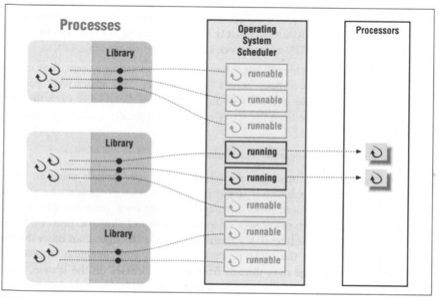
\includegraphics[scale=0.6]{kernel_level_threads.png}\\
  Fig 1 : Kernel level threads
\end{center} 


The advantages and disadvantages are briefly listed below :-

Advantages
\begin{enumerate}
\item Because kernel has full knowledge of all threads, scheduler may decide to give more time to a process having large number of threads than process having small number of threads. While in user-level thread kernel have no idea about the number of threads present in the processes. 
\item True parallelism is possible as the threads of the same process can run on multiple cores simultaneosuly.
\item Kernel-level threads are especially good for applications that frequently block.
\end{enumerate}

Disadvantages
\begin{enumerate}
\item The kernel-level threads are slow and inefficient. For instance, threads operations are hundreds of times slower than that of user-level threads.
\item Thread management is more expensive in case of kernel level threads as they involve system calls.
\item Scheduling is now bound to the scheduling algorithm within the kernel. The user level scheduling and the choice to implement a different scheduling algorithm at the process level is not available.
\end{enumerate}

\subsection{Hybrid approaches}
Since user level threads and kernel level threads are two extreme approaches to thread management, there are other approaches that try to bridge the gap between the idea of user and kernel level threads.

\subsubsection{Scheduler activation}
This is similar to user-level threads with the assumption that kernel has some information about the threads in the process. It also allows communication between process and kernel i.e. you can pass information back and forth between process and kernel. So, basically in this case kernel level scheduler and user-level library scheduler collaborate to achieve some goals rather than each making decisions independently without the knowledge of the other. For example, when user-level thread makes a system call the process blocks but you can inform kernel that there are more threads. This avoids the blocking of entire process. Similarly, you can notify user-level library if I/O is completed. The library scheduler may inform the kernel scheduler
when it creates or deletes a thread within a process. This can be seen as a N:M mapping i.e. N user-level threads getting mapped to M kernel entities compared to 1:1 mapping in kernel-level threads and N:1 mapping in user-level threads. 

\subsubsection{Light-weight processes}
This is also an intermediate model between user-level and kernel level threads. Light-weight processes or LWPs is an abstract concept that allows a many-to-many mapping between the threads and scheduler. Each process contains one or more LWP, each of which runs one or more user threads. Here, kernel level scheduler schedules the light weight processes  and if an LWP mapped to multiple threads is chosen to execute, the user level scheduler will schedule one of the threads for execution. Each LWP is a kernel resource in a kernel pool, and is allocated (attached) and de-allocated (detached) to a thread on a per thread basis. This happens as threads are scheduled or created and destroyed. System level calls are required to instantiate new LWPs.\\

\begin{center}
  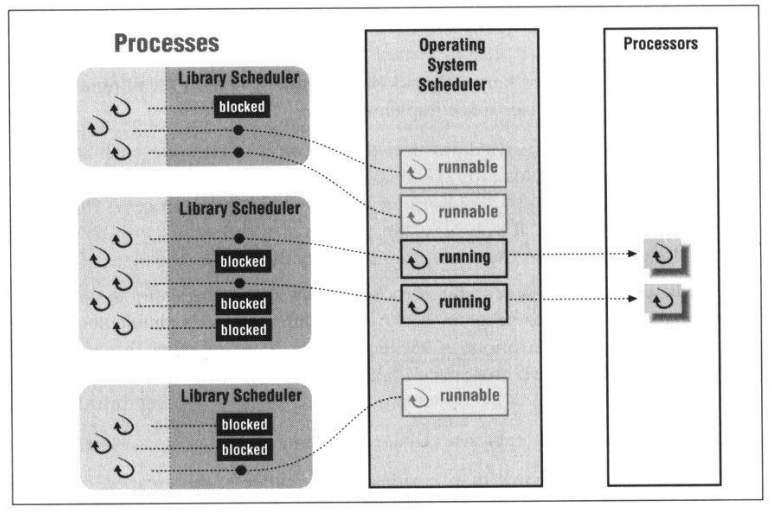
\includegraphics[scale=0.6]{light_weight_processes.png}\\
  Fig 2 : Light-weight processes example
\end{center} 

Solaris is one of the operating systems that follows this model.


\section{Thread packages}

\subsection{POSIX threads}
POSIX is a standard interface that can be used using C/C++ build multi-threaded applications. It is cross-platform which means that if an OS or library supports POSIX threads, the code can be ported, recomplied and run on a that platform. Also, the POSIX standard does not mention anything about the implementation of the interface. As a result, there are user-level as well as kernel-level implementations of Pthreads. 

\subsection{Java threads}
Java threads are native to the language. Therefore, every JVM supports Java threads. Similar to POSIX, Java threads do not require a specific JVM implementation and user-level as well as kernel-level thread implementations exist.

\section{Multi-processor scheduling}
In a multi-processor scenario, there are N processors in the system. Every processor/core has a set caches like the L1 cache, L2 cache etc. The function of a cache is to save frequently and recently accessed instructions or data for fast access as compared to fetching them from the memory. These caches are not shared across processors. Each processor/core has its own L1/L2 cache. In some cases, caches are shared but here we assume the simple case where caches are not shared. Processors use system bus to communicate with memory. Multi-processor scheduling involves scheduling tasks in such an environment.  

There are two variants for the multi-processor scheduling implmentaiton.

\subsection{Central queue}
 The most basic approach is to simply
reuse the basic framework for single processor scheduling, by putting all
jobs that need to be scheduled into a single or global queue. Whenever a processor goes idle, the CPU scheduler runs on that processor and schedules a process/thread from this queue. This approach has the advantage of simplicity; it does not require much work to take an
existing policy that picks the best job to run next and adapt it to work on
more than one CPU. 

Since the processors are independent of each other, there can be a case where two or more processors go idle at the same time. A clear disadvantage of sharing a single queue amongst processors is that the processor requires a locking mechanism before unloading a task from the queue and this may prove to become a bottleneck and slow the scheduling down beacuse at a time only one processor can acquire the lock so other processors have to wait, this will lead of wastage of CPU cycles on these processors. As the number of processors increase, the probability of lock contention increases and the system spends more and more time in lock overhead and less time doing the work the system should be doing. 

The second main problem with central queue is cache affinity. Because each CPU simply picks the next job to run from the globally shared
queue, each job ends up bouncing around from CPU to CPU, thus
doing exactly the opposite of what would make sense from the standpoint
of cache affinity. There would be lot of cache misses in this case which will dramatically reduce performance.

\subsection{Distributed queue}
In this approach, there are multiple task queues each of which may be shared by multiple processors. In an extreme case, there could be a queue per processor which may also be called its local queue. Whenever a processor goes idle, its scheduling algorithm examines its local queue only to schedule a task to that processor.

Distributed queue has a distinct advantage over Central queue in that it should be inherently
more scalable. As the number of CPUs grows, so too does the number
of queues, and thus lock and cache contention should not become a
central problem. In addition, this intrinsically provides cache affinity;
jobs stay on the same CPU and thus reap the advantage of reusing cached
contents therein.

It is possible that the queues are unbalanced when compared to each other i.e. the number of tasks in the local queue of one processor may be significantly more than the number of tasks in the queue of another processor. In that case, they may be load balanced periodically if required. 

\textbf{Question}: What if during load balancing some tasks are transferred from one queue to another?\\
\textbf{Answer}: Yes, that is possible and then the process will again start from cold cache but the key idea is load balancing happens far less frequently than the times the process actually runs. So, that's an acceptable price to pay to get better performance due to cache affinity and load balancing. \\

\textbf{Question}: If you terminate a process and start a new version of that program, does that cover cahe affinity?\\
\textbf{Answer}: Cache affinity is specific to a process. If you restart a process,  there will be new address space, new data, new code, so you won't be able to take advantage of cache affinity even if it is the same code. \\

\textbf{Question}: Who does the load balancing?\\
\textbf{Answer}: That's the job of CPU scheduler.\\

\textbf{Question}: What to do if some queues are emptying faster than other queues?\\
\textbf{Answer}: For all active processes, you would try to balance the queues. If some queues are emptying faster, you would reassign some other processes to that queue. \\

So, there are couple of things to keep in mind while scheduling on multiprocessors:
1. Exploit cache affinity: Try to schedule on the same
processor that a process/thread executed last. 
2. Pick larger quantum sizes to decrease context switch overhead. 



\subsection{Gang scheduling}
In the global and distributed queue implementations, the processors schedule tasks independent of what is being executed on other processors. There may be cases where we may desire true parallelism out of an application i.e. all the threads of a process should run simultaneosuly. 

A class of schedulers known as gang schedulers allow the mentioned behaviour by coordinating the scheduling of threads withn a process on different processors. The threads of a process are scheduled in a ``gang'' or group on different cores/processors. This improves the performance of the parallel application. Gang scheduling is only useful for massively parallel applications, this is not used for general purpose scheduling.


\section{Distributed scheduling}
In a distributed system, there may be N independent machines connected to each other over a network. If a machine is overloaded or operating at its maximum capacity, an incoming task on that machine may be run on a different machine in the system and its results can be sent back to the original machine. The goal of distributed scheduling is to maximize the use of all resources in a system. Just like multiprocessor scheduling schedules thread on more than one core, distributed scheduling schedules a pool of job on more than one machine. Distributed scheduling makes sense only if the probability that there is at least one system idle and at least one job waiting is high enough.

If the system is lightly loaded (low utilization), the probability that any given machine in the system is idle is high. This implies that a job entering a system will most probably be able to be executed on the same machine without transferring it to some other machine in the system. In case of a heavily loaded system(high utilization), the likelihood that every machine in the system is saturated is high and the chances of finding an idle machine are low. If a new job arrives in this system, the probability that it will have to wait is high. In both of these cases, distributed scheduling is not feasible because the probability that there is at least one system idle and at least one job waiting is low in both these cases.

Therefore, distributed scheduling is useful only when the system is moderately utilized i.e. the case when the load on a local machine is high enough and the chances to find an idle machine are also high enough.

\textbf{Question}: How is Distributed scheduling different from Multiprocessor scheduling?\\
\textbf{Answer}: In Multiprocessor scheduling the memory is shared, all the processes you are trying to run are loaded on one machine, you are just scheduling them on different cores of the machine. While in Distributed scheduling if a job is running on machine I and you decide it to run on machine J, there is a lot more work required to transfer its memory state. Its far more expensive to make the decision to run on other machine in Distributed scheduling while in Multiprocessor scheduling you didn't have to move anything, its already running on that machine.  \\

\subsection{Design Issues}
{\bf Load}: CPU queue lengths and CPU utilization are good indicators of load.\\
{\bf Policy}: Static(decisions hard-wired into scheduling algorithm using prior knowledge of system), Dynamic( use state information to make decisions) and  Adaptive (special case of dynamic algorithms; dynamically change parameters of the scheduling algorithm)\\
{\bf Preemptive vs. Nonpreemptive}: Preemptive transfers -- transfer of a task that is partially executed, expensive due to collection of task's state, Nonpreemptive transfers -- only transfer tasks that have not begun execution. Preemptive schedulers are more flexible but at the same time more complicated. \\
{\bf Centralized vs. Decentralized}: Centralized -- The decision to send a job made globally, Decentralized - the decision is made locally in this case.\\
{\bf Stability}: For stability, the departure rate should be higher than arrival rate or there should be some kind of load balancing else the system will get heavily loaded.

\subsection{Components of Scheduler}
{\bf Transfer Policy}: It is used to determine that a node is in a suitable state to participate in a task
transfer. Mostly, threshold-based to classify nodes as senders, receivers, or OK. It determines if a process should be executed remotely or locally\\
{\bf Selection Policy}: It determines which task should be transfered from a node. The simplest is to select a newly arrived task that have caused the node
to become a sender. The task selected for transfer should be such so that the overhead from
task transfer is compensated by a reduction is task's response time.\\
{\bf Location Policy}: It determines which node should get the task selected for transfer. This is done by polling
(serially or in parallel). A node can be selected for polling randomly , based on
information from previous polls, or on a nearest-neighbor manner.\\
{\bf Information Policy}: It determines when should the information of other nodes should be collected; demand-driven, or periodic, or state-change-driven.\\

\subsection{Sender-initiated Distributed Scheduler }
The overloaded node attempts to send tasks to lightly loaded node.
\begin{itemize}
\item {\bf Transfer policy}: CPU queue threshold T for all nodes. Initiated when a queue length exceeds T.
\item {\bf Selection policy}: newly arrived tasks only. 
\item {\bf Location policy}:
\begin{itemize}
\item Random: select any node to transfer the task at random. The selected node X
may be overloaded. If transferred task is treaded as new arrival, then X may
transfer the task again. Limit the transfers for a task. Is effective under lightload
conditions.
\item Threshold: Poll nodes until a receiver is found. Up to PollLimit nodes are polled.
If none is a receiver, then the sender commits to the task.
\item Shortest: Among the polled nodes that were found to be receivers, select the
one with the shortest queue. Marginal improvement.
\end{itemize}
\item {\bf Information policy}: demand-driven, initiated by the sender.
\item {\bf Stability}: Unstable at high-loads
\end{itemize}


\subsection{Receiver-initiated Distributed Scheduler }

The underloaded node attempts to receive tasks from heavily loaded node.
\begin{itemize}
\item {\bf Transfer policy}: when a task departs, node compares its CPU queue length is
compared with T, and if smaller, node is a receiver.
\item {\bf Selection policy}:  newly arrived or partially executed
process
\item {\bf Location policy}:
\begin{itemize}
\item Random: Randomly poll nodes until a sender is found, and transfer a
task from it. If no sender is found, wait for a period or until a task completes,
and repeat.
\item Threshold: Poll nodes until a sender is found. Up to PollLimit nodes are polled.
If none is a sender, then do nothing.
\item Shortest: Among the polled nodes that where found to be sender, select the
one with the heaviest load. 
\end{itemize}
\item {\bf Information policy}: demand-driven, initiated by the receiver.
\item{\bf  Stability}: At high loads, a receiver will find a sender with high-probability
with a small number of polls. At low-loads, most polls will fail, but this is
not a problem, since CPU cycles are available.
\item {\bf Disadvantage}: CPU scheduling algorithms are mostly round-robin, so a newly
arrived task at an overload node is quickly given a slice and this starts
execution. Thus, very likely preemptive transfer of tasks will take place. 
\end{itemize}

\subsection{Symmetrically-initiated Distributed Scheduler }
It combines both sender-initiated and receiver-initiated
components in order to get a hybrid algorithm with the
advantages of both. Care must be taken since otherwise, the hybrid algorithm may
inherit the disadvantages of both sender and receiver initiated
algorithms. In improved version, it maintains receiver, sender and OK nodes using the polling information. 

\section{Case Study}
\subsection{V-System}
It uses state-change driven information policy i.e. broadcast information when there is significant change in CPU/memory utilization. It implements a sender-initiated algorithm which maintains a list of M least loaded nodes(receivers). While off-loading, it probes random receiver from M and transfers job only if it is still a receiver. This doesn't mean that sender will send all its jobs to the receiver, only one job is off- loaded at a time. 

\subsection{Sprite}
This also uses state-change driven information policy and implements a sender-initiated scheduling algorithm. There is a centralized coordinator which keeps the status of load on all the machines. They made an assumption that if there is no mouse or keyboard activity for 30 seconds and the number of active processes is less than a threshold it becomes a receiver. Foreign processes get terminated when the user returns. It also implemented process migration so that the process can continue running from its last state. For process migration, the entire memory contents as well as kernel state has to transferred to other machine. There are many problems with process migration e.g. I/O, network communication.

\textbf{Question}: Can process migration cause huge overhead?\\
\textbf{Answer}: It absolutely will cause huge overhead. Larger the process, larger the memory you have to transfer.\\

 
\end{document}
